\documentclass[aspectratio=169,11pt]{beamer}

\usepackage[T1]{fontenc}
\usepackage[utf8]{inputenc}
\usepackage{libertine}
\usepackage[sfdefault]{sourcesanspro}
\usepackage{microtype}
\usepackage{tikz}
\usetikzlibrary{positioning,calc,arrows.meta}
\usepackage{booktabs}
\usepackage{graphicx}
\usepackage{xcolor}

\definecolor{paper}{HTML}{FBF9F5}
\definecolor{ink}{HTML}{14212E}
\definecolor{muted}{HTML}{6E7B85}
\definecolor{rule}{HTML}{DCD5C8}
\definecolor{teal}{HTML}{14636B}
\definecolor{clay}{HTML}{A6503A}
\definecolor{tint}{HTML}{F1EEE7}

\hypersetup{
  pdftitle={How Do Global Shocks Affect Australia? A summary of RBA RDP 2024-10},
  pdfauthor={Patrick Hendy and Benjamin Beckers},
  pdfsubject={Summary deck of Reserve Bank of Australia Research Discussion Paper 2024-10},
  pdfkeywords={global spillovers, global financial cycle, banks, Australia, FAVAR}
}
\title{How Do Global Shocks Affect Australia?}
\author{Patrick Hendy and Benjamin Beckers}
\date{December 2024}

\setbeamertemplate{navigation symbols}{}
\setbeamercolor{background canvas}{bg=paper}
\setbeamercolor{normal text}{fg=ink}
\setbeamercolor{structure}{fg=teal}
\setbeamercolor{foot}{fg=muted,bg=paper}
\setbeamersize{text margin left=1.0cm,text margin right=1.0cm}

\setlength{\parindent}{0pt}
\setlength{\parskip}{0pt}
\hyphenpenalty=10000
\exhyphenpenalty=10000

\def\decksource{}
\newcommand{\src}[1]{\def\decksource{#1}}

\setbeamertemplate{footline}{%
  \begin{beamercolorbox}[wd=\paperwidth,ht=0.72cm,dp=0.04cm,leftskip=1.0cm,rightskip=1.0cm]{foot}%
    {\color{rule}\rule{\dimexpr\paperwidth-2.0cm\relax}{0.35pt}}\par
    \vspace{0.10cm}%
    {\fontsize{6.8}{8.4}\selectfont\color{muted}\decksource\hfill\insertframenumber}%
  \end{beamercolorbox}%
}

\newcommand{\kicker}[1]{%
  {\fontsize{7.6}{9}\selectfont\color{teal}\bfseries\textls[130]{\MakeUppercase{#1}}}\par
  \vspace{0.16cm}}
\newcommand{\headline}[1]{%
  {\rmfamily\fontsize{18.4}{21.8}\selectfont\color{ink}#1\par}
  \vspace{0.34cm}}
\newcommand{\bodyfont}{\fontsize{9.7}{12.9}\selectfont}
\newcommand{\smallfont}{\fontsize{8.2}{11.2}\selectfont}
\newcommand{\notefont}{\fontsize{7.1}{9.4}\selectfont}
\newcommand{\leadin}[1]{{\bfseries\color{teal}#1}}
\newcommand{\rulebreak}{\par\vspace{0.16cm}{\color{rule}\rule{\linewidth}{0.35pt}}\par\vspace{0.16cm}}

\begin{document}

% ---------------------------------------------------------------- 1. title
\begin{frame}[plain]
\vspace*{0.95cm}
{\fontsize{7.8}{10}\selectfont\color{teal}\bfseries\textls[130]{RESERVE BANK OF AUSTRALIA \enspace·\enspace RESEARCH DISCUSSION PAPER 2024-10}}\par
\vspace{1.55cm}
{\rmfamily\fontsize{29}{34}\selectfont\color{ink} How Do Global Shocks\\[0.08cm] Affect Australia?\par}
\vspace{0.64cm}
{\color{teal}\rule{3.2cm}{1.5pt}}\par
\vspace{0.48cm}
{\fontsize{12.2}{15}\selectfont\color{ink} Patrick Hendy and Benjamin Beckers\par}
\vspace{0.14cm}
{\fontsize{8.8}{11}\selectfont\color{muted} Economic Research Department, December 2024\par}
\vfill
{\fontsize{7.8}{10}\selectfont\color{muted} A summary deck prepared from the published paper \hfill doi.org/10.47688/rdp2024-10\par}
\vspace{0.78cm}
\end{frame}

% ---------------------------------------------------------------- 2. question
\begin{frame}[t]
\src{Hendy \& Beckers (2024), RDP 2024-10}
\vspace*{0.42cm}
\kicker{1 \enspace·\enspace The question}
\headline{Small, open and fully exposed --- how much does it actually matter?}
\bodyfont

\begin{minipage}[t]{8.45cm}
\raggedright
Australia is a small open economy with open capital markets. Global shocks reach it quickly, and
policy must decide how much weight to give them.

\vspace{0.30cm}
The evidence disagrees: foreign shocks have been estimated to explain 20 to over 50 per cent of
Australian GDP variation, and 10 to 70 per cent of the exchange rate.

\vspace{0.30cm}
And the channel is contested: trade, the exchange rate, asset prices, or global banks.
\end{minipage}\hfill
\begin{minipage}[t]{5.15cm}
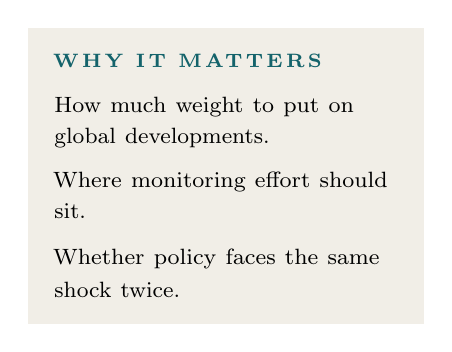
\begin{tikzpicture}[baseline={(current bounding box.north)}]
\node[fill=tint, inner sep=0.34cm, text width=4.35cm, align=left, anchor=north west] at (0,0) {%
  {\fontsize{7.2}{9}\selectfont\color{teal}\bfseries\textls[130]{WHY IT MATTERS}}\par
  \vspace{0.18cm}
  {\smallfont
  How much weight to put on global developments.\par
  \vspace{0.16cm}
  Where monitoring effort should sit.\par
  \vspace{0.16cm}
  Whether policy faces the same shock twice.}
};
\end{tikzpicture}
\end{minipage}
\end{frame}

% ---------------------------------------------------------------- 3. approach
\begin{frame}[t]
\src{Section 1; Section 3}
\vspace*{0.42cm}
\kicker{2 \enspace·\enspace Approach}
\headline{A FAVAR lets the data define ``global'', not assume it means ``American''.}
\bodyfont

Most Australian studies put US variables in the foreign block. That misses shocks which reach
Australia without passing through the United States --- an Asian financial crisis, for instance.

\vspace{0.28cm}
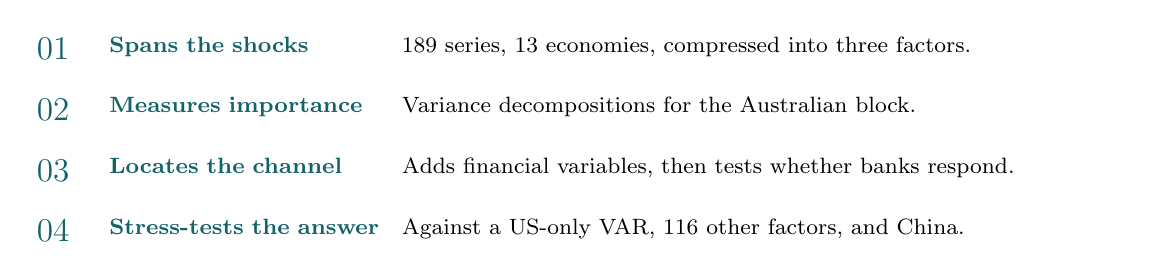
\begin{tikzpicture}[x=1cm,y=1cm,baseline={(current bounding box.north)}]
\foreach \y/\n/\lead/\text in {%
  0/01/Spans the shocks/{189 series, 13 economies, compressed into three factors.},
  -0.77/02/Measures importance/{Variance decompositions for the Australian block.},
  -1.54/03/Locates the channel/{Adds financial variables, then tests whether banks respond.},
  -2.31/04/Stress-tests the answer/{Against a US-only VAR, 116 other factors, and China.}}
{
  \node[anchor=north west, font=\fontsize{13}{15}\selectfont\color{teal}] at (0,\y) {\n};
  \node[anchor=north west, text width=3.55cm, align=left, font=\smallfont] at (0.92,\y+0.02) {\leadin{\lead}};
  \node[anchor=north west, text width=9.0cm, align=left, font=\smallfont] at (4.65,\y+0.02) {\text};
}
\end{tikzpicture}
\end{frame}

% ---------------------------------------------------------------- 4. method
\begin{frame}[t]
\src{Section 3.1; Section 3.1.2}
\vspace*{0.42cm}
\kicker{3 \enspace·\enspace Method}
\headline{Two stages: extract global factors, then estimate a small VAR.}
\bodyfont

{\centering
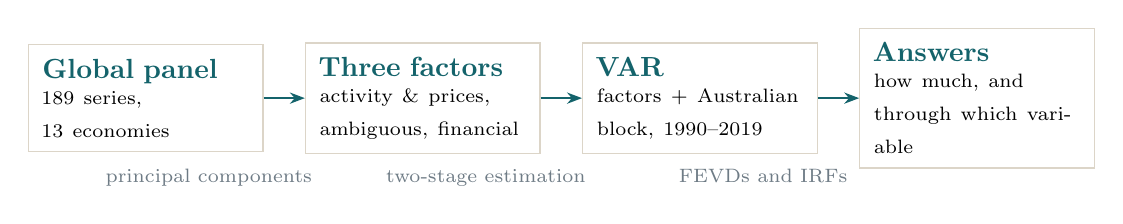
\begin{tikzpicture}[x=1cm,y=1cm,baseline={(current bounding box.north)},
  box/.style={draw=rule, line width=0.45pt, fill=white, text width=2.62cm,
  minimum height=1.22cm, align=left, inner sep=0.18cm, anchor=west},
  lab/.style={font=\fontsize{6.9}{8.4}\selectfont\color{muted}}]
\node[box] (a) at (0,0) {{\bfseries\color{teal}Global panel}\\[0.02cm]{\fontsize{7.4}{8.8}\selectfont 189 series,\\ 13 economies}};
\node[box] (b) at (3.52,0) {{\bfseries\color{teal}Three factors}\\[0.02cm]{\fontsize{7.4}{8.8}\selectfont activity \& prices,\\ ambiguous, financial}};
\node[box] (c) at (7.04,0) {{\bfseries\color{teal}VAR}\\[0.02cm]{\fontsize{7.4}{8.8}\selectfont factors + Australian\\ block, 1990--2019}};
\node[box] (d) at (10.56,0) {{\bfseries\color{teal}Answers}\\[0.02cm]{\fontsize{7.4}{8.8}\selectfont how much, and\\ through which variable}};
\draw[-{Stealth[length=1.9mm]}, color=teal, line width=0.7pt] (a.east) -- (b.west);
\draw[-{Stealth[length=1.9mm]}, color=teal, line width=0.7pt] (b.east) -- (c.west);
\draw[-{Stealth[length=1.9mm]}, color=teal, line width=0.7pt] (c.east) -- (d.west);
\node[lab, anchor=north] at (2.30,-0.78) {principal components};
\node[lab, anchor=north] at (5.82,-0.78) {two-stage estimation};
\node[lab, anchor=north] at (9.34,-0.78) {FEVDs and IRFs};
\end{tikzpicture}\par}

\vspace{0.30cm}
{\smallfont
\leadin{Australian block} CPI inflation, the cash rate, unemployment, the TWI and real GDP.\par
\vspace{0.15cm}
\leadin{Small open economy} Australian variables cannot move the global factors, on impact or with a
lag.\par
\vspace{0.15cm}
\leadin{Sample} Quarterly 1990--2019, excluding COVID. The factors are not structural.\par}
\end{frame}

% ---------------------------------------------------------------- 5. factors
\begin{frame}[t]
\src{Section 3.1.3; Table B1; Figure 3}
\vspace*{0.42cm}
\kicker{4 \enspace·\enspace The factors}
\headline{Three factors capture about 30 per cent of the global panel --- very unevenly.}
\bodyfont

\begin{minipage}[t]{8.0cm}
\raggedright
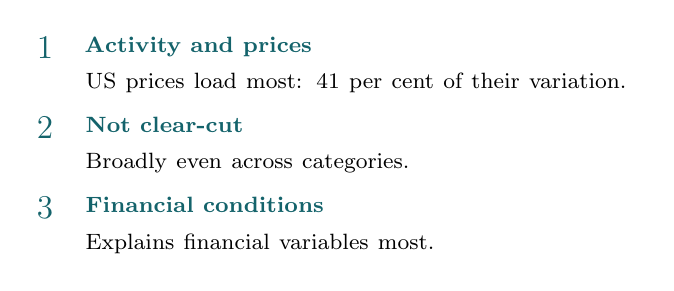
\begin{tikzpicture}[x=1cm,y=1cm,baseline={(current bounding box.north)}]
\foreach \y/\n/\lead/\text in {%
  0/1/{Activity and prices}/{US prices load most: 41 per cent of their variation.},
  -1.02/2/{Not clear-cut}/{Broadly even across categories.},
  -2.04/3/{Financial conditions}/{Explains financial variables most.}}
{
  \node[anchor=north west, font=\fontsize{12}{14}\selectfont\color{teal}] at (0,\y) {\n};
  \node[anchor=north west, text width=7.0cm, align=left] at (0.62,\y) {%
    {\smallfont\bfseries\color{teal}\lead}\par\vspace{0.04cm}{\smallfont\text}};
}
\end{tikzpicture}

\vspace{0.30cm}
{\smallfont
The factors are orthogonal and carry no economic label: they summarise common variation, not identified
shocks. Three were chosen by the Bai--Ng criteria.}
\end{minipage}\hfill
\begin{minipage}[t]{5.3cm}
{\notefont\color{muted}\bfseries\textls[100]{AVERAGE VARIATION EXPLAINED}}\par
\vspace{0.22cm}
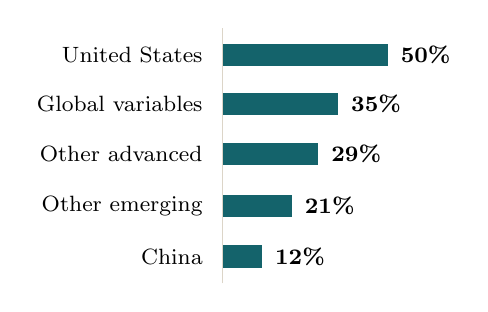
\begin{tikzpicture}[x=1cm,y=1cm,baseline={(current bounding box.north)}]
\foreach \y/\lab/\val in {0/{United States}/50, -0.62/{Global variables}/35, -1.26/{Other advanced}/29, -1.92/{Other emerging}/21, -2.56/{China}/12}
{
  \node[anchor=east, font=\smallfont] at (2.55,\y) {\lab};
  \fill[teal] (2.68,\y-0.14) rectangle ({2.68+\val*0.042},\y+0.14);
  \node[anchor=west, font=\smallfont\bfseries] at ({2.72+\val*0.042},\y) {\val\%};
}
\draw[rule, line width=0.35pt] (2.68,-2.90) -- (2.68,0.34);
\end{tikzpicture}

\vspace{0.08cm}
\end{minipage}
\end{frame}

% ---------------------------------------------------------------- 6. headline
\begin{frame}[t]
\src{Figure 5, redrawn; values at a 16-quarter horizon}
\vspace*{0.42cm}
\kicker{5 \enspace·\enspace How much}
\headline{Global shocks explain half of the cash rate and the exchange rate, a sixth of GDP.}
\bodyfont

\begin{minipage}[t]{8.75cm}
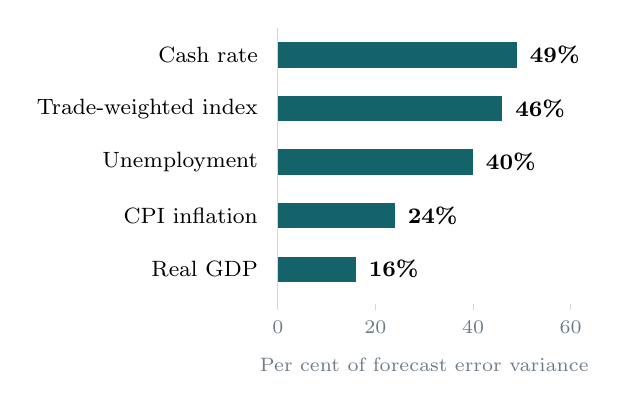
\begin{tikzpicture}[x=1cm,y=1cm,baseline={(current bounding box.north)}]
\foreach \y/\lab/\val in {0/{Cash rate}/49, -0.68/{Trade-weighted index}/46, -1.36/{Unemployment}/40, -2.04/{CPI inflation}/24, -2.72/{Real GDP}/16}
{
  \node[anchor=east, font=\smallfont] at (3.05,\y) {\lab};
  \fill[teal] (3.18,\y-0.16) rectangle ({3.18+\val*0.062},\y+0.16);
  \node[anchor=west, font=\smallfont\bfseries] at ({3.22+\val*0.062},\y) {\val\%};
}
\draw[rule, line width=0.35pt] (3.18,-3.16) -- (3.18,0.34);
\foreach \t in {0,20,40,60}
{
  \draw[rule, line width=0.3pt] ({3.18+\t*0.062},-3.16) -- ({3.18+\t*0.062},-3.24);
  \node[anchor=north, font=\notefont\color{muted}] at ({3.18+\t*0.062},-3.26) {\t};
}
\node[anchor=north, font=\notefont\color{muted}] at (5.04,-3.72) {Per cent of forecast error variance};
\end{tikzpicture}
\end{minipage}\hfill
\begin{minipage}[t]{4.45cm}
\raggedright
{\smallfont
Global shocks dominate the two variables that are supposed to absorb them, and matter much less
for output.

\vspace{0.28cm}
The gap between the exchange rate and GDP is the paper's central quantitative result --- and the
reason the next question, through what, matters.\par}
\end{minipage}
\end{frame}

% ---------------------------------------------------------------- 7. interpretation
\begin{frame}[t]
\src{Section 4.1.1; Figure 6}
\vspace*{0.42cm}
\kicker{5 \enspace·\enspace How much}
\headline{That pattern is what a buffered economy looks like.}
\bodyfont

\begin{minipage}[t]{6.7cm}
\raggedright
\leadin{The dollar moves first.}\\[0.03cm]
{\smallfont
The TWI reprices within a quarter and stays there, as efficient markets would predict. It takes the
shock so domestic activity does not have to.\par}

\vspace{0.30cm}
\leadin{The cash rate moves later.}\\[0.03cm]
{\smallfont
It responds gradually, consistent with the RBA updating its outlook slowly or adjusting in steps.
Either way, policy offsets the shock rather than passing it on.\par}
\end{minipage}\hfill
\begin{minipage}[t]{6.1cm}
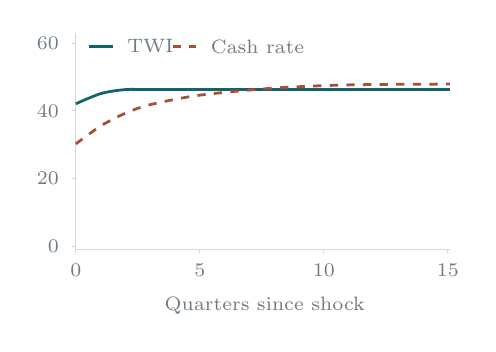
\begin{tikzpicture}[x=1cm,y=1cm,baseline={(current bounding box.north)}]
\draw[rule, line width=0.35pt] (0.55,0) -- (0.55,2.75);
\draw[rule, line width=0.35pt] (0.55,0) -- (5.30,0);
\foreach \v in {0,20,40,60}
  {\draw[rule, line width=0.3pt] (0.50,{0.04+\v*0.043}) -- (0.55,{0.04+\v*0.043});
   \node[anchor=east, font=\notefont\color{muted}] at (0.46,{0.04+\v*0.043}) {\v};}
\foreach \q in {0,5,10,15}
  {\draw[rule, line width=0.3pt] ({0.55+\q*0.315},{0}) -- ({0.55+\q*0.315},{-0.04});
   \node[anchor=north, font=\notefont\color{muted}] at ({0.55+\q*0.315},-0.06) {\q};}
\draw[teal, line width=1.0pt] plot[smooth] coordinates {(0.55,1.85)(0.87,1.98)(1.18,2.03)(1.50,2.03)(2.45,2.03)(5.30,2.03)};
\draw[clay, line width=1.0pt, dashed] plot[smooth] coordinates {(0.55,1.34)(0.87,1.57)(1.18,1.73)(1.50,1.84)(2.13,1.96)(3.08,2.05)(4.03,2.09)(5.30,2.10)};
\draw[teal, line width=1.0pt] (0.72,2.58) -- (1.02,2.58);
\node[anchor=west, font=\notefont\color{muted}] at (1.08,2.58) {TWI};
\draw[clay, line width=1.0pt, dashed] (1.78,2.58) -- (2.08,2.58);
\node[anchor=west, font=\notefont\color{muted}] at (2.14,2.58) {Cash rate};
\node[anchor=north, font=\notefont\color{muted}] at (2.95,-0.48) {Quarters since shock};
\end{tikzpicture}
\end{minipage}

\rulebreak
{\smallfont
\leadin{What is left is composition, not collapse.} GDP held up through the 2001 US recession and the
GFC while unemployment still rose, and the pain was regional: mining-exposed Western Australia and
Queensland held up while New South Wales deteriorated.\par}
\end{frame}

% ---------------------------------------------------------------- 8. US VAR
\begin{frame}[t]
\src{Section 4.1.2; Figure 7, redrawn; values at a 16-quarter horizon}
\vspace*{0.42cm}
\kicker{6 \enspace·\enspace Robustness}
\headline{A US-only VAR does nearly as well.}
\bodyfont

\begin{minipage}[t]{9.55cm}
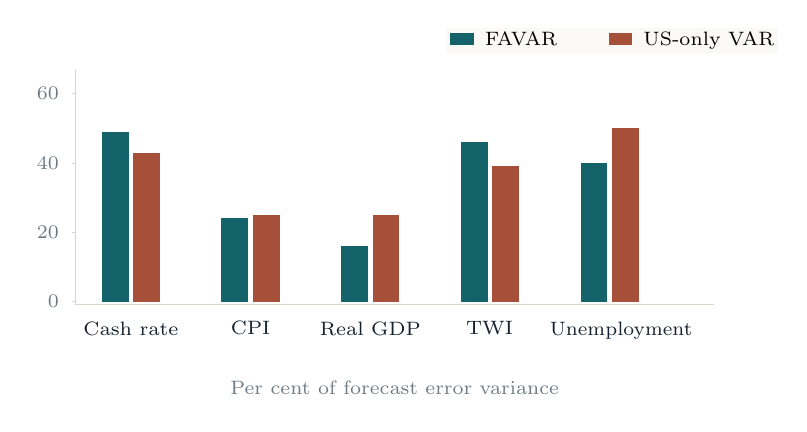
\begin{tikzpicture}[x=1cm,y=1cm,baseline={(current bounding box.north)}]
\draw[rule, line width=0.35pt] (0.85,0) -- (0.85,2.98);
\draw[rule, line width=0.35pt] (0.85,0) -- (8.95,0);
\foreach \v in {0,20,40,60}
  {\draw[rule, line width=0.3pt] (0.80,{0.04+\v*0.044}) -- (0.85,{0.04+\v*0.044});
   \node[anchor=east, font=\notefont\color{muted}] at (0.76,{0.04+\v*0.044}) {\v};}
\foreach \i/\lab/\favar/\us in {0/{Cash rate}/49/43, 1/{CPI}/24/25, 2/{Real GDP}/16/25, 3/{TWI}/46/39, 4/{Unemployment}/40/50}
{
  \pgfmathsetmacro{\x}{1.55+\i*1.52}
  \fill[teal] ({\x-0.37},0.04) rectangle ({\x-0.03},{0.04+\favar*0.044});
  \fill[clay] ({\x+0.03},0.04) rectangle ({\x+0.37},{0.04+\us*0.044});
  \node[anchor=north, font=\notefont\color{ink}, align=center, text width=1.52cm] at (\x,-0.09) {\lab};
}
\node[anchor=north, font=\notefont\color{muted}] at (4.9,-0.84) {Per cent of forecast error variance};
\node[anchor=west, font=\notefont, fill=paper, inner sep=0.05cm] at (5.55,3.36) {\textcolor{teal}{\rule{0.30cm}{0.15cm}}\enspace FAVAR \qquad \textcolor{clay}{\rule{0.30cm}{0.15cm}}\enspace US-only VAR};
\end{tikzpicture}
\end{minipage}\hfill
\begin{minipage}[t]{3.95cm}
\raggedright
{\smallfont
The FAVAR explains more of the cash rate and the TWI, about the same of unemployment, and less of
CPI and GDP.

\vspace{0.26cm}
None of the differences is statistically significant.

\vspace{0.26cm}
Over 1990--2019, US variables were effectively a sufficient statistic for the global shocks that
mattered here.\par}
\end{minipage}
\end{frame}

% ---------------------------------------------------------------- 9. extra factors / China
\begin{frame}[t]
\src{Section 4.1.3--4.1.4; Figures 8--10}
\vspace*{0.42cm}
\kicker{6 \enspace·\enspace Robustness}
\headline{A fourth factor adds little --- and the best ones are Chinese.}
\bodyfont

\begin{minipage}[t]{8.4cm}
\raggedright
Principal components explain the global panel, not Australia. So the paper swaps the fourth component
for each of 116 alternatives.

\vspace{0.30cm}
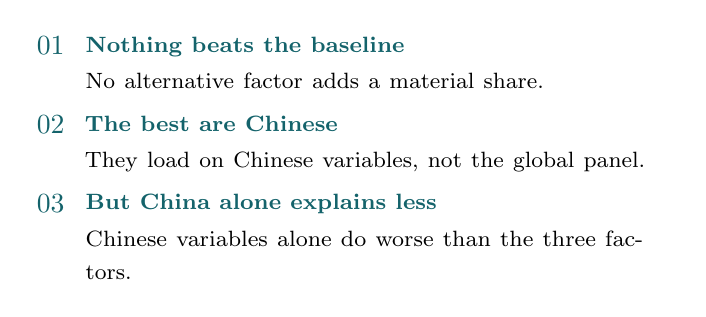
\begin{tikzpicture}[x=1cm,y=1cm,baseline={(current bounding box.north)}]
\foreach \y/\n/\lead/\text in {%
  0/01/{Nothing beats the baseline}/{No alternative factor adds a material share.},
  -1.00/02/{The best are Chinese}/{They load on Chinese variables, not the global panel.},
  -2.00/03/{But China alone explains less}/{Chinese variables alone do worse than the three factors.}}
{
  \node[anchor=north west, font=\fontsize{10}{12}\selectfont\color{teal}] at (0,\y) {\n};
  \node[anchor=north west, text width=7.4cm, align=left] at (0.62,\y) {%
    {\smallfont\bfseries\color{teal}\lead}\par\vspace{0.04cm}{\smallfont\text}};
}
\end{tikzpicture}
\end{minipage}\hfill
\begin{minipage}[t]{4.9cm}
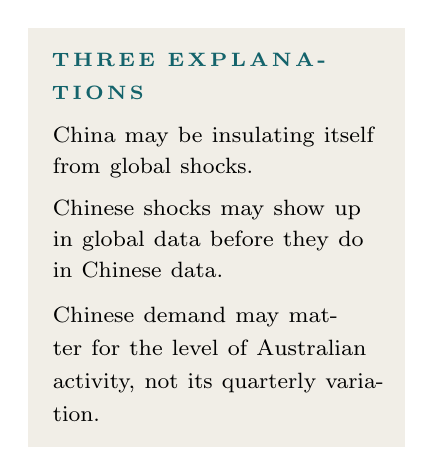
\begin{tikzpicture}[baseline={(current bounding box.north)}]
\node[fill=tint, inner sep=0.32cm, text width=4.15cm, align=left, anchor=north west] at (0,0) {%
{\fontsize{7.2}{9}\selectfont\color{teal}\bfseries\textls[130]{THREE EXPLANATIONS}}\par
\vspace{0.16cm}
{\smallfont
China may be insulating itself from global shocks.\par
\vspace{0.14cm}
Chinese shocks may show up in global data before they do in Chinese data.\par
\vspace{0.14cm}
Chinese demand may matter for the level of Australian activity, not its quarterly variation.}\par
};
\end{tikzpicture}
\end{minipage}
\end{frame}

% ---------------------------------------------------------------- 10. where it lands
\begin{frame}[t]
\src{Section 5.1; Figure 11, redrawn; values at a 16-quarter horizon}
\vspace*{0.42cm}
\kicker{7 \enspace·\enspace Channels}
\headline{Asset prices take the shock. Bank balance sheets barely move.}
\bodyfont

\begin{minipage}[t]{6.55cm}
{\notefont\color{teal}\bfseries\textls[130]{ASSET PRICES}}\par
\vspace{0.20cm}
{\rmfamily\fontsize{27}{31}\selectfont\color{ink}55\%}\par
{\smallfont\color{muted} of the variation in the ASX all ordinaries\par}
\vspace{0.22cm}
{\rmfamily\fontsize{27}{31}\selectfont\color{ink}40\%}\par
{\smallfont\color{muted} of the variation in housing prices\par}
\vspace{0.24cm}
{\smallfont Stock prices adjust on impact; housing prices build up over time, consistent with a
slow-moving market or an effect intermediated by the cash rate.}
\end{minipage}\hfill
\begin{minipage}[t]{6.35cm}
{\notefont\color{muted}\bfseries\textls[130]{BANK BALANCE SHEETS}}\par
\vspace{0.22cm}
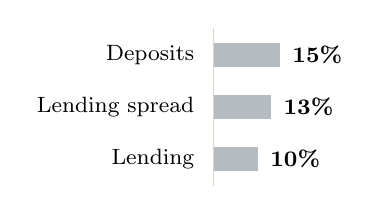
\begin{tikzpicture}[x=1cm,y=1cm,baseline={(current bounding box.north)}]
\foreach \y/\lab/\val in {0/{Deposits}/15, -0.66/{Lending spread}/13, -1.32/{Lending}/10}
{
  \node[anchor=east, font=\smallfont] at (2.70,\y) {\lab};
  \fill[muted!50] (2.82,\y-0.15) rectangle ({2.82+\val*0.056},\y+0.15);
  \node[anchor=west, font=\smallfont\bfseries] at ({2.86+\val*0.056},\y) {\val\%};
}
\draw[rule, line width=0.35pt] (2.82,-1.66) -- (2.82,0.34);
\end{tikzpicture}

\vspace{0.24cm}
{\smallfont
Around a tenth to a sixth of the variation, with confidence bands that span zero. If banks were the
channel, these are the variables that should move.}
\end{minipage}
\end{frame}

% ---------------------------------------------------------------- 11. IRF
\begin{frame}[t]
\src{Section 5.2; Figure 12, redrawn; central estimate and 68 per cent band at 16 quarters}
\vspace*{0.42cm}
\kicker{7 \enspace·\enspace Channels}
\headline{Shock the financial factor: prices move, bank quantities do not.}
\bodyfont

\begin{minipage}[t]{9.45cm}
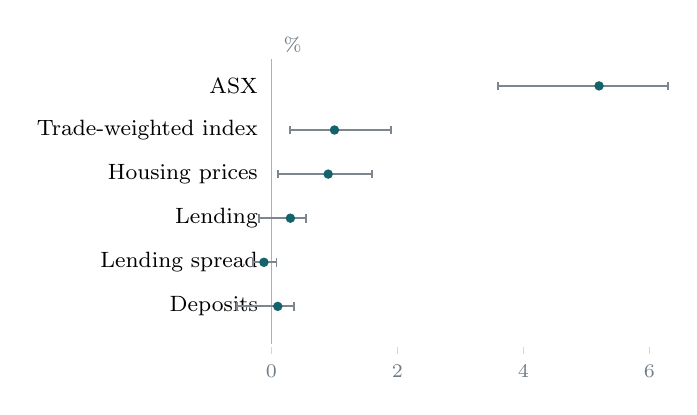
\begin{tikzpicture}[x=1cm,y=1cm,baseline={(current bounding box.north)}]
\draw[ink!35, line width=0.5pt] (3.00,0.34) -- (3.00,-3.28);
\node[anchor=south west, font=\notefont\color{muted}] at (3.03,0.30) {\%};
\foreach \t in {0,2,4,6}
{
  \pgfmathsetmacro{\xx}{3.00+\t*0.80}
  \draw[rule, line width=0.3pt] (\xx,-3.40) -- (\xx,-3.32);
  \node[anchor=north, font=\notefont\color{muted}] at (\xx,-3.42) {\t};
}
\foreach \y/\lab/\c/\lo/\hi in {%
  0/{ASX}/5.2/3.6/6.3,
  -0.56/{Trade-weighted index}/1.0/0.3/1.9,
  -1.12/{Housing prices}/0.9/0.1/1.6,
  -1.68/{Lending}/0.3/-0.2/0.55,
  -2.24/{Lending spread}/-0.12/-0.30/0.08,
  -2.80/{Deposits}/0.10/-0.55/0.35}
{
  \pgfmathsetmacro{\xlo}{3.00+\lo*0.80}
  \pgfmathsetmacro{\xhi}{3.00+\hi*0.80}
  \pgfmathsetmacro{\xc}{3.00+\c*0.80}
  \node[anchor=east, font=\smallfont] at (2.95,\y) {\lab};
  \draw[ink!55, line width=0.7pt] (\xlo,\y) -- (\xhi,\y);
  \draw[ink!55, line width=0.7pt] (\xlo,\y-0.055) -- (\xlo,\y+0.055);
  \draw[ink!55, line width=0.7pt] (\xhi,\y-0.055) -- (\xhi,\y+0.055);
  \fill[teal] (\xc,\y) circle (0.06);
}
\end{tikzpicture}
\end{minipage}\hfill
\begin{minipage}[t]{4.05cm}
\raggedright
{\smallfont
A one standard deviation shock to the factor that loads on financial variables lifts the ASX by about
5 per cent and the TWI by about 1 per cent.

\vspace{0.26cm}
Lending, deposits and spreads end the horizon close to zero, with bands that straddle it.

\vspace{0.26cm}
That is what a channel that is \emph{not} operating looks like.\par}
\end{minipage}
\end{frame}

% ---------------------------------------------------------------- 12. why insulated
\begin{frame}[t]
\src{Section 6.1; Figures 13--17}
\vspace*{0.42cm}
\kicker{8 \enspace·\enspace Why}
\headline{Why Australian banks are insulated: three structural reasons.}
\bodyfont

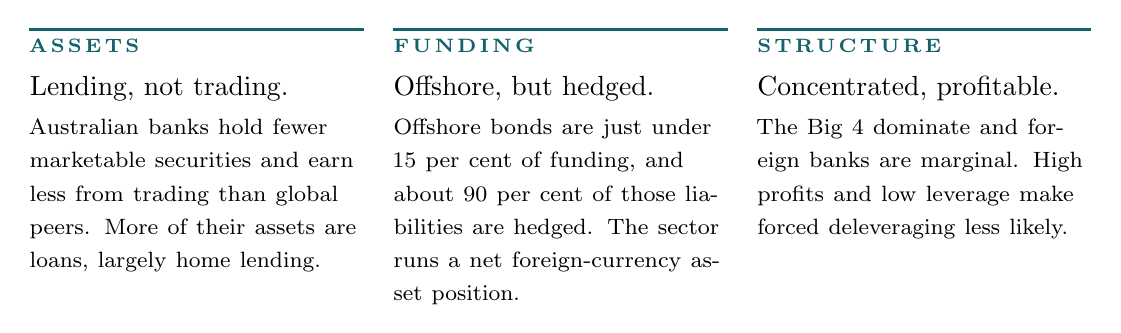
\begin{tikzpicture}[x=1cm,y=1cm,baseline={(current bounding box.north)}, card/.style={text width=4.25cm, align=left, anchor=north west, inner sep=0cm}]
\foreach \x/\tg/\lead/\text in {%
  0/{ASSETS}/{Lending, not trading.}/{Australian banks hold fewer marketable securities and earn less from trading than global peers. More of their assets are loans, largely home lending.},
  4.62/{FUNDING}/{Offshore, but hedged.}/{Offshore bonds are just under 15 per cent of funding, and about 90 per cent of those liabilities are hedged. The sector runs a net foreign-currency asset position.},
  9.24/{STRUCTURE}/{Concentrated, profitable.}/{The Big 4 dominate and foreign banks are marginal. High profits and low leverage make forced deleveraging less likely.}}
{
  \draw[teal, line width=1.1pt] (\x,0.02) -- (\x+4.25,0.02);
  \node[card] at (\x,-0.10) {%
    {\fontsize{7.1}{9}\selectfont\color{teal}\bfseries\textls[130]{\tg}}\par
    \vspace{0.12cm}
    {\fontsize{9.6}{11.6}\selectfont\lead}\par
    \vspace{0.08cm}
    {\fontsize{7.9}{10.6}\selectfont\text}\par};
}
\end{tikzpicture}

\vspace{0.24cm}
\rulebreak
{\smallfont
\leadin{The counter-argument.} Concentration can also amplify a shock concentrated in one major bank
--- a too-big-to-fail dynamic rather than a buffer.\par}
\end{frame}

% ---------------------------------------------------------------- 13. what transmits
\begin{frame}[t]
\src{Section 5; Appendix C, Figure C1}
\vspace*{0.42cm}
\kicker{7 \enspace·\enspace Channels}
\headline{The channels that do transmit look traditional.}
\bodyfont

\begin{tabular}{@{}p{2.75cm} p{1.65cm} p{8.35cm}@{}}
\toprule
{\notefont\color{muted}CHANNEL} & {\notefont\color{muted}STRENGTH} & {\notefont\color{muted}EVIDENCE} \\
\midrule
\rule{0pt}{0.52cm}{\bfseries Exchange rate} & {\color{rule}\rule{1.20cm}{1.6pt}}\hspace{-1.20cm}{\color{teal}\rule{1.20cm}{1.6pt}} & About 46 per cent of TWI variation, within a quarter. \\
\rule{0pt}{0.52cm}{\bfseries Asset prices} & {\color{rule}\rule{1.20cm}{1.6pt}}\hspace{-1.20cm}{\color{teal}\rule{1.20cm}{1.6pt}} & 55 per cent for the ASX, 40 per cent for housing. \\
\rule{0pt}{0.50cm}{\bfseries Trade} & {\color{rule}\rule{1.20cm}{1.6pt}}\hspace{-1.20cm}{\color{teal}\rule{0.68cm}{1.6pt}} & About 30 per cent for the terms of trade. \\
\rule{0pt}{0.52cm}{\bfseries Banking} & {\color{rule}\rule{1.20cm}{1.6pt}}\hspace{-1.20cm}{\color{teal}\rule{0.18cm}{1.6pt}} & 10--15 per cent; the bands span zero. \\
\bottomrule
\end{tabular}

\vspace{0.40cm}
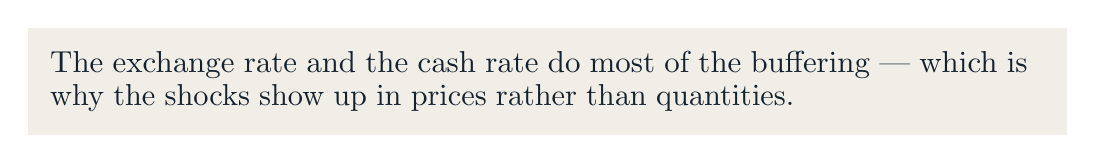
\begin{tikzpicture}[baseline={(current bounding box.north)}]
\node[fill=tint, inner sep=0.30cm, text width=12.6cm, align=left, anchor=north west] at (0,0) {%
{\rmfamily\fontsize{10.8}{13.4}\selectfont\color{ink}The exchange rate and the cash rate do most of
the buffering --- which is why the shocks show up in prices rather than quantities.}\par
};
\end{tikzpicture}
\end{frame}

% ---------------------------------------------------------------- 14. implications
\begin{frame}[t]
\src{Section 6.2; Section 7}
\vspace*{0.42cm}
\kicker{9 \enspace·\enspace Implications}
\headline{The banking channel is a feature of a financial system, not a law.}
\bodyfont

\begin{minipage}[t]{6.55cm}
{\notefont\color{teal}\bfseries\textls[130]{FOR POLICY}}\par
\vspace{0.24cm}
\leadin{Monitor the right link.}\\[0.03cm]
{\smallfont
If spillovers arrive through the exchange rate, trade and asset prices, that is where scenario work
belongs.\par}
\vspace{0.24cm}
\leadin{Do not import another country's channel.}\\[0.03cm]
{\smallfont
The global-banking result is about internationalised, trading-heavy systems.\par}
\vspace{0.24cm}
\leadin{Structure is endogenous.}\\[0.03cm]
{\smallfont
The features that muted the channel here are shaped by regulation. Change them and the answer can
change.\par}
\end{minipage}\hfill
\begin{minipage}[t]{6.2cm}
{\notefont\color{teal}\bfseries\textls[130]{FOR RESEARCH}}\par
\vspace{0.24cm}
\leadin{A selection problem.}\\[0.03cm]
{\smallfont
Spillovers are identified from heterogeneity in foreign exposures, so the countries that can be
estimated may be exactly where the channel is strongest.\par}
\vspace{0.24cm}
\leadin{Test it where the structure differs.}\\[0.03cm]
{\smallfont
Systems like Australia's are the useful case: an absent channel where theory says it should be weak is
evidence about the channel itself.\par}
\end{minipage}
\end{frame}

% ---------------------------------------------------------------- 15. limits + takeaways
\begin{frame}[t]
\src{Section 1; Section 3; Section 7}
\vspace*{0.42cm}
\kicker{10 \enspace·\enspace Limits and takeaways}
\headline{What this design cannot say --- and what it does.}
\bodyfont

\begin{minipage}[t]{6.3cm}
{\notefont\color{muted}\bfseries\textls[130]{LIMITS}}\par
\vspace{0.20cm}
{\smallfont
\leadin{The sample stops in 2019.} A linear framework cannot absorb COVID, and the paper does not claim
the 1990--2019 mix of shocks will repeat.\par
\vspace{0.18cm}
\leadin{The factors are not structural.} They identify that a shock is global, not which shock it is.\par
\vspace{0.18cm}
\leadin{No long-run identification.} China may matter for levels in a way quarterly variation cannot
reveal.\par
\vspace{0.18cm}
\leadin{One country, one structure.} This is evidence about Australia, and a prompt to compare banking
systems --- not a theorem about small open economies.\par}
\end{minipage}\hfill
\begin{minipage}[t]{6.45cm}
{\notefont\color{muted}\bfseries\textls[130]{THREE TAKEAWAYS}}\par
\vspace{0.20cm}
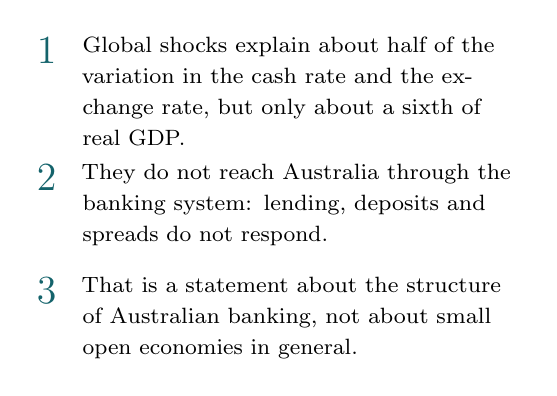
\begin{tikzpicture}[x=1cm,y=1cm,baseline={(current bounding box.north)}]
\foreach \y/\n/\text in {%
  0/1/{Global shocks explain about half of the variation in the cash rate and the exchange rate, but only about a sixth of real GDP.},
  -1.62/2/{They do not reach Australia through the banking system: lending, deposits and spreads do not respond.},
  -3.05/3/{That is a statement about the structure of Australian banking, not about small open economies in general.}}
{
  \node[anchor=north west, font=\fontsize{15}{17}\selectfont\color{teal}] at (0,\y) {\n};
  \node[anchor=north west, text width=5.55cm, align=left, font=\smallfont] at (0.58,\y+0.01) {\text};
}
\end{tikzpicture}
\end{minipage}
\end{frame}

% ---------------------------------------------------------------- 16. source
\begin{frame}[t]
\src{}
\vspace*{0.42cm}
\kicker{Source}
\headline{The paper.}
\bodyfont

\begin{minipage}[t]{8.7cm}
\raggedright
{\fontsize{9.9}{12.8}\selectfont
Hendy, P and B Beckers (2024), ``How Do Global Shocks Affect Australia?'', \emph{Research Discussion
Paper} 2024-10, Economic Research Department, Reserve Bank of Australia, December.\par}

\vspace{0.40cm}
{\notefont\color{muted}
DOI: \texttt{doi.org/10.47688/rdp2024-10}\par
\vspace{0.08cm}
PDF: \texttt{rba.gov.au/publications/rdp/2024/pdf/rdp2024-10.pdf}\par
\vspace{0.08cm}
JEL: C38, F36, F42\par
\vspace{0.08cm}
Keywords: global spillovers, global financial cycle, banks\par}

\vspace{0.90cm}
{\notefont\color{muted}
Charts are redrawn from the paper's Figures 3, 5, 7, 11 and 12, with values read from the published
figures and rounded. The paper and its figures are published by the Reserve Bank of Australia under a
Creative Commons Attribution 4.0 International licence; the views are the authors' and not those of
the RBA.\par}
\end{minipage}\hfill
\begin{minipage}[t]{4.9cm}
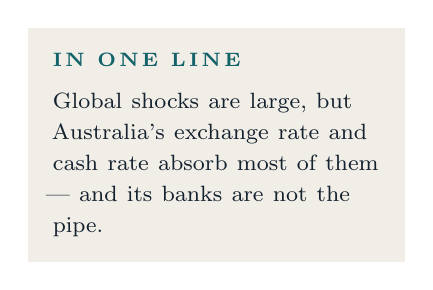
\begin{tikzpicture}[baseline={(current bounding box.north)}]
\node[fill=tint, inner sep=0.32cm, text width=4.15cm, align=left, anchor=north west] (p) at (0,0) {%
{\fontsize{7.2}{9}\selectfont\color{teal}\bfseries\textls[130]{IN ONE LINE}}\par
\vspace{0.14cm}
{\smallfont\color{ink}
Global shocks are large, but Australia's exchange rate and cash rate absorb most of them --- and its
banks are not the pipe.\par}
};
\end{tikzpicture}
\end{minipage}
\end{frame}

\end{document}
